% source: https://tex.stackexchange.com/questions/133183/draw-spiral-cone-tikz


\documentclass[dvipsnames]{article}
\usepackage{pgfplots}
\usetikzlibrary{decorations.markings}
\pgfplotsset{compat=newest}

\def\Point{36.9}

\begin{document}

\pagenumbering{gobble}


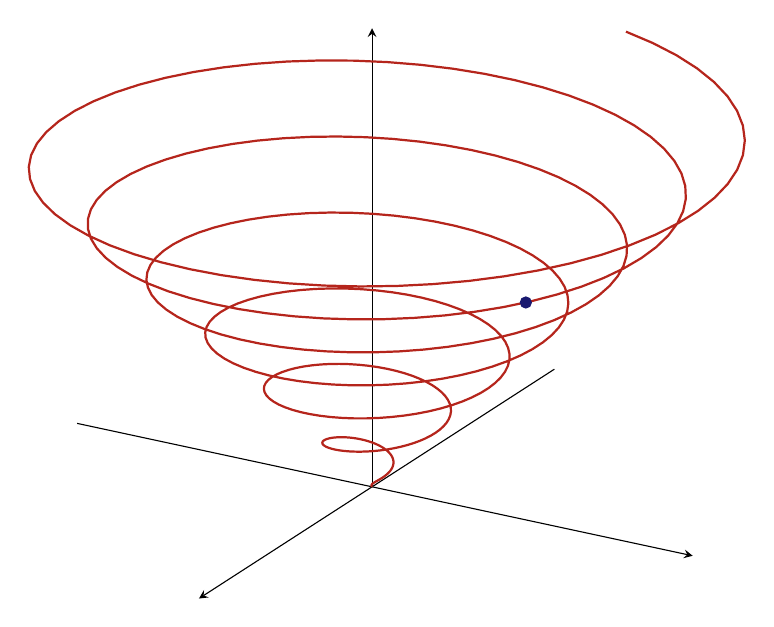
\begin{tikzpicture}
\begin{axis}[
 view={-30}{-30},
 axis lines=middle,
 zmax=60,
 height=12cm,
 xtick=\empty,
 ytick=\empty,
 ztick=\empty
]
\addplot3+[,ytick=\empty,yticklabel=\empty,
  mark=none,
  thick,
  BrickRed,
  domain=0:14.7*pi,
  samples=400,
  samples y=0,
]
({x*sin(0.28*pi*deg(x))},{x*cos(0.28*pi*deg(x)},{x});
\addplot3+[
  mark options={color=MidnightBlue},
  mark=*
]
coordinates {({\Point*sin(0.28*pi*deg(\Point))},{\Point*cos(0.28*pi*deg(\Point)},{\Point})};
% \addplot3+[
%   mark=none,
%   dashed,
%   domain=0:12*pi,
%   samples=100,
%   samples y=0
% ]
({\Point*sin(0.28*pi*deg(\Point))},{\Point*cos(0.28*pi*deg(\Point)},{x});
% \addplot3[
%   mark=none,
%   dashed
% ]
coordinates {(0,0,0) ({\Point*sin(0.28*pi*deg(\Point))},{\Point*cos(0.28*pi*deg(\Point)},{0})};

% \draw[
% radius=80,
% decoration={
%   markings,
%   mark= at position 0.99 with {\arrow{latex}}
%   },
% postaction=decorate
% ]
(axis cs:0,10,0) arc[start angle=80,end angle=14] (axis cs:14,0,0);
% \node at (axis cs:20,0,30) {$P$};
% \node at (axis cs:20,17,0) {$\rho$};
% \node at (axis cs:24,0,7) {$z$};
% \node at (axis cs:7,12,0) {$\phi$};
\end{axis}
\end{tikzpicture}

\end{document}
